\newpage

\section{Структура системы автоматической имитации возраста}

\subsection{Описание конвеера имитации возраста}

Любая система имитации возраста состоит из двух компонентов:
\begin{enumerate}
\item Получение текущего возраста фото
\item Синтез нового лица по следующим данным: фото, текущий возраст, изменённый возраст
\end{enumerate}
Текущий возраст фото может быть как задан пользователем, так и получен с помощью одного из алгоритмов оценки возраста.
Во втором случае на вход алгоритму поступает изображение, а на выходе получается одно число: либо конкретный возраст (если оценка возраста решает задачу регрессии), либо возрастная группа (если решается задача классификации).

В качестве алгоритма оценки возраста в конвеере используется алгоритм CNN Age Classification \cite{cnn_age_gender}, описанный ранее в разделе <<Автоматическое определение возраста>>. Данный алгоритм принимает на вход изображение лица, масштабирует его до размеров, совпадающих с размером входного слоя нейросети, затем выполняет прямой проход по нейросети и получает значения на нескольких выходах нейросети, по одному на каждый возрастной кластер. Результирующим кластером считается тот, который имеет наибольшее значение на своём выходе.
Код, загружающий изображение в нейросеть, написан на Python, проход по нейросети выполняется с помощью фреймворка Caffe. Изображение передаётся через файл, скрипту на Python передаётся имя файла. Номер результирующего кластера выдаётся в стандартный вывод.

Второй компонент конвеера, синтезирующий лица, построим на основе техник, описанных в статье Illumination-Aware Age Progression. Данный алгоритм взят за основу как наиболее актуальный из рассмотренных ранее. Кроме того, данный алгоритм, в отличие от Gandhi, полностью автоматический.

Общая схема работы этого алгоритма выглядит так:
\begin{enumerate}
\item Получение фото
\item Выравнивание фото
\item Имитация текстурных изменений
\item Имитация изменений в оптическом потоке
\item Коррекция пропорций лица
\end{enumerate}

Этап выравнивания фото будет подробно описан далее.

Имитация текстурных изменений включает в себя:
\begin{enumerate}
  \item Вычисление <<переосвещённых>> (relightable) средниx $ A^I_s $ и $ A^I_t $ для целевого и текущего кластеров
  \item Вычисление оптического потока $ F_{source-input} $ от $ A^I_s $ к $I$, \\
   $ J_s $ - искривление (warping) $ A^I_s $ c помощью этого потока
  \item Вычисление оптического потока $ F_{target-input} $ от $ A^I_t $ к $I$, \\
  $ J_t $ - искривление (warping) $ A^I_t $ c помощью этого потока
  \item Наложение на исходное изображение I текстурной разницы: \\
   $ I' = J_t - J_s $
\end{enumerate}

Имитация изменений в оптическом потоке по сути является преобразованием $I'$ с помощью потока $F_{target-source}$.
Коррекция пропорций лица осуществляется путём растягивания (интерполяции) изображения с исходного размера до нового, с исправленными пропорциями.

\subsection{Описание конвеера обучения}

Перед тем, как можно будет приступать к имитации возраста, необходимо вычислить оптические потоки $F_{target-source}$ для всех возможных пар $(target, source)$, на каждом $i$-м кластере получить $ V_i $ для вычисления relightable-изображений и вычислить средние пропорции лица.

Чтобы сделать это, необходимо обучающую выборку изображений также пропустить через конвейер. Структура этого конвеера следующая:
\begin{enumerate}
  \item Разбиение изображений на фиксированные кластеры по возрасту
  \item Выравнивание изображений внутри кластера
  \item Вычисление матриц $ V_i $ для каждого i-го кластера на основе выровненных изображений методом главных компонент
  \item Для каждой пары кластеров $ (A_i, A_j) $ таких, что $ i < j $:
  \begin{enumerate}
    \item для каждого $I_k$, такого, что $ I_k \in \lbrace A_i \cap A_j \rbrace $, вычислить $ A_i^k, A_j^k $
    \item сформировать многоканальные изображения $ \bold{A}_i , \bold{A}_j $  из одноканальных $ A_i^k, A_j^k $
    \item Пользуясь многоканальным алгоритмом поиска оптического потока, найти оптический поток $F_{j-i}$
  \end{enumerate}
\end{enumerate}

\hyphenation{Simple-Flow}

Одним из подходящих алгоритмов для вычисления оптического потока на изображении с произвольным числом каналов является SimpleFlow \cite{simple_flow}. В основе метода SimpleFlow лежит очевидная идея поиска в локальной окрестности каждого пикселя наиболее похожий на него пиксель. Для разрешения неоднозначностей и для компенсации шумов делается предположение, что в окрестности данного пикселя все точки имеют почти одинаковый сдвиг. Кроме того, поиск происходит на пирамиде изображений с увеличением масштаба на каждом уровне в два раза.

Алгоритм не использует значения пикселей непосредственно, а лишь сравнивает их между собой. Следовательно, алгоритм способен работать на изображении, состоящем из пикселей любого вида, если только для каждой пары пикселей задана функция расстояния $ d(x, y) $ между ними.

\subsection{Методы выравнивания}

Цель этапа выравнивания --- получить изображения лиц, как можно более близкие к т.н. нейтральному выражению лица. Нейтральное выражение лица как правило задаётся неким фиксированным положением ключевых точек на изображении, например, установленным вручную (см. рис. \ref{fig:neutral}).

\begin{figure}[t]
	\centering
	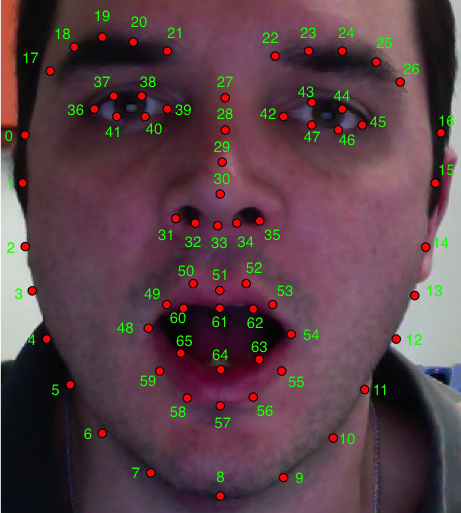
\includegraphics[width=0.3\textwidth]{avatar-annotation.png}
	\caption{Пример нейтрального расположения ключевых точек}
	\label{fig:neutral}
\end{figure}

Ещё один способ задать положение ключевых точек --- запустить один из детекторов ключевых точек на образцовой фотографии. При этом лицо на фотографии не должно выражать никаких эмоций, должно быть расположено строго анфас и ровно освещено (это желательно для работы детектора ключевых точек). Достоинство такого подхода --- во взаимозаменяемости детекторов. Недостатки --- в том, что положение точек привязывается к конкретному лицу и в том, что при детектировании ключевых точек ошибка может быть весьма серьёзной. Тем не менее данный подход используется в статье Frontalization \cite{frontalization}, а вместо фотографии используется сгенерированное (rendered) изображение 3d-модели, для целей, указанных в статье, этого вполне достаточно.

Один из способов сравнить между собой различные способы выравнивания --- определить на каждом выровненном изображении новые координаты ключевых точек и сравнивать эти координаты между собой. Однако, такой объём работы подразумевает полную переразметку всей базы тестовых изображений. В то же время поручить эту задачу детектору ключевых точек означало бы внести в измерения дополнительную ошибку, связанную с точностью детектора.

Однако, цель выравнивания изображения состоит, очевидно, в том, чтобы определённые черты лица находились в строго определённых позициях на изображении. Следовательно, если для всех выровненных изображений вычислить среднее, то при корректном выравнивании мы получим изображение лица, размытое внутри отдельных его черт, однако, с чёткими границами между чертами лица.

Для того, чтобы оценить степень размытости, введём метрику средней магнитуды: будем измерять градиент среднего изображения. Для каждого канала вычислим градиенты с помощью алгоритма Собеля, и посчитаем средний модуль градиентов по всем каналам.

Далее описаны методы выравнивания, которые были реализованы и протестированы в ходе проведения данной работы.

\subsubsection{Collection flow}

Авторы статьи Illumination-aware Age Progression \cite{illumination_aware} выполняют входное выравнивание с помощью собственного алгоритма Collection flow \cite{collection_flow}.
 
Данный алгоритм вычисляет плотный оптический поток между парами лиц на заданной коллекции изображений лиц.
Для этого для каждого изображения из коллекции делается следующее:

\begin{enumerate}
  \item Изображение проецируется на подпространство низкой размерности с целью получить нейтральное выражение лица
  \item От исходного изображения к проекции вычисляется оптический поток
\end{enumerate}

Затем исходят из предположения о нулевом оптическом потоке между нейтральными выражениями лица и для каждой пары изображений объединяют оптические потоки: сначала поток от исходного изображения к нейтральному, затем обратный поток от конечного изображения к нейтральному.

Алгоритм использует некоторые наблюдения за подходом Eigenfaces, в котором производится анализ коллекции изображений лиц методом главных компонент. Авторы исходят из предположения, что несколько первых главных компонент кодируют изменения в яркости отдельных черт лица, а также глобальные условия освещения. В то же время главные компоненты с меньшими собственными числами кодируют изменения в выражении и форме лица.

Это происходит из-за того, что так называемое non-rigid face motion, т.е. изменение выражения лица, состоит из следующих изменений изображения:

\begin{enumerate}
  \item Изменения в оптическом потоке (проявляются только на границах частей лица)
  \item Изменение формы частей лица, т.е. изменение нормалей (проявляются только на выпуклостях и впадинах)
  \item Изменения, связанные с заслонением одних частей лица другими (в виде анфас это только рот и глаза)
\end{enumerate}

Как видим, все эти изменения крайне разреженные, т.е. они касаются лишь отдельных небольших областей на лице. В то же время изменение освещённости (например, яркость, цвет или положение источника освещения) затрагивает практически всё лицо. А поскольку проекция лица rank-4, т.е. на подпространство из 4 главных компонент сохраняет до 90\% вариаций, то в основном в первых главных компонентах оказываются изменения изображения, связанные с освещением, если только исходная коллекция лиц была богата на различные режимы освещения.

Если эти предположения справедливы, то проецирование на подпространство из первых нескольких собственных векторов должно удалять с лица все различия в выражении. Однако, на практике такая низкоранговая проекция (low-rank projection) размывает лицо, на нём теряются мелкие детали, что дольно плохо для optical flow, поскольку алгоритму становится сложнее сравнивать между собой локальные окрестности точек.

Чтобы устранить данный эффект, для каждого изображения запускается итерационный алгоритм:
\begin{enumerate}
  \item Устанавливаем число главных компонент $ k = 4 $, для каждого изображения $ i $ инициализируем оптический поток $ F_i $ нулями (тождественное преобразование), помещаем в матрицу M все изображения $ I_i $
  \item Вычисляем проекции $ I_i' $ из матрицы $M$ c использованием первых $k$ главных компонент
  \item Вычисляем оптический поток $ F_i' $ от $I_i$ до $I_i'$, добавляем его к $ F_i $
  \item Искривляем $ I_i $ с использованием потока $ F_i' $
  \item $ k := k + 1 $
  \item Если норма L2 разности потоков $ F_i $ на текущей итерации и на предыдущей больше, чем фиксированный порог (в статье указан порог 20), то переходим к шагу 2, иначе останавливаемся
\end{enumerate}

Такой подход вычисления оптического потока по утверждению авторов хорошо справляется с различиями в освещении, альбедо, условиях съёмки, баланса белого и т.д., и в то же время приводит выражения лиц к нейтральному виду.

Кроме того, он позволяет вычислить оптический поток для всех изображений в коллекции за время $ O(n) $, а не за время $ O(n^2) $, как это было бы при попарном вычислении оптического потока.

\subsubsection{Фронтализация} 

В статье Effective Face Frontalization in Unconstrained Images \cite{frontalization} предлагается новый подход к генерации изображения с исправленным ракурсом. Авторы используют детектор ключевых точек, чтобы найти ключевые точки на входном изображении и сопоставить их с ключевыми точками на изображении образцового лица, для которого известна его точная 3d-модель. Используя эти данные, ищется поза лица в пространстве, после чего трёхмерная модель вписывается в изображение лица и генерируется изображение головы во фронтальной позе. Для восстановления частей изображения, заслонённых из-за поворота головы (например, одна из сторон носа), используется зеркально симметричная копия изображения (см. рис. \ref{fig:frontal2}).

В подробностях алгоритм выглядит следующим образом:
\begin{enumerate}
\item Пусть задано образцовое лицо, а именно:
\begin{itemize}
	\item Изображение $ I_R $, являющееся проекцией трёхмерной модели нейтрального лица
	\item Массив точек $ P = \{ P_i = (X_i, Y_i, Z_i)^T \}_{i=1}^N $ модели, проецирующихся в пиксели  $ p'_i = (x'_i, y'_i)^T  $ для всех пикселей изображения $ I_R $
	\item Массив ключевых точек $ K = \{ K_j = (X_j, Y_j, Z_j)^T \}_{j=1}^M $, проецирущихся в пиксели $ k'_j = (x'_j, y'_j)^T  $ для всех ключевых точек, найденных на изображении $ I_r $ выбранным алгоритмом поиска ключевых точек
	\item Матрица камеры $ A_R $, с помощью которой осуществлялось проецирование 3d-точек на плоскость:
	$$
	z'_i \begin{bmatrix} x'_i \\ y'_i \\ 1 \end{bmatrix}  = M_R P_i, M_R = A_R [R_R t_R],
	$$
где $ R_R $ и $ t_R $ --- соответственно матрица поворота и вектор трансляции в 3d-пространстве, $ z'_i $ --- масштабный коэффициент
\end{itemize} 
\item Найти на входном изображении $I_Q$ ключевые точки \\
$ b' = \{ b'_j = (x'_j, y'_j, 1)^T \}_{j=1}^M $ выбранным алгоритмом поиска ключевых точек
\item Найти матрицу проекции $ M_Q = A_R \left [ R_Q t_Q \right ] $ такую, что 
$$
M_Q = \argmin_{M_Q} \lbrace M_Q K - z^T b' \rbrace,
$$
где $ R_Q, t_Q $ --- соответственно матрица поворота и вектор трансляции в 3d-пространстве, $ z $ --- вектор-столбец неизвестных масштабных коэффициентов
\item С помощью матрицы $ M_Q $ спроецировать массив точек $ P $ на плоскость, получив набор 2d-точек $ p_Q $
\item Вычислить карту заслонений $ O_Q $:
\begin{enumerate}
	\item для каждого пикселя исходного изображения посчитать кол-во спроецированных туда точек из $p_Q$
	\item размыть $ O_Q $ гауссовым фильтром
\end{enumerate}
\item Создать новое изображение $ I_F $, перенести значения из пикселей $ p_Q $ изображения $I_Q$ в пиксели $p'$ изображения $I_F$
\item Проделать аналогичную операцию с $O_Q$, получив $O_F$
\item Использовать веса из $O_Q$ для заполнения заслонённых частей изображения, используюя симметрично отображённую копию $I_Q$ как источник
\end{enumerate}

\begin{figure}[t]
	\centering
	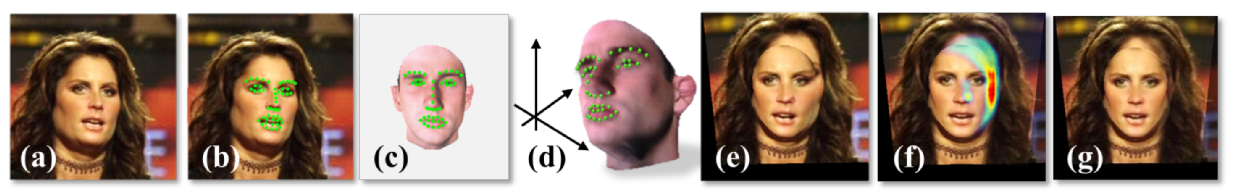
\includegraphics[width=\textwidth]{frontal2.png}
	\caption{Последовательность операций во время фронтализации}
	\label{fig:frontal2}
\end{figure}

Данный алгоритм не занимается непосредственно нейтрализацией выражения лица, однако, может быть предварять работу других алгоритмов.

\subsubsection{Искривление по ключевым точкам}

Выравнивание фото по ключевым точкам подразумевает следующую последовательность действий:
\begin{enumerate}
  \item Детектирование набора ключевых точек на лице
  \item Кадрирование лица по ключевым точкам
  \item Искривление изображения с целью выравнить позу лица
\end{enumerate}

Алгоритмы поиска ключевых точек на лице как правило основываются на двух компонентах: модель формы и модель внешнего вида. В ходе поиска ключевых точек алгоритм из начального приближения начинает итеративный поиск наилучшего расположения точек на лице, чередуя два этапа: коррекция результата с точки зрения модели формы и коррекция результата с точки зрения модели внешнего вида. Коррекция формы находит наилучшее приближение текущего расположения точек параметрами модели. Коррекция же по внешнему виду для каждой ключевой точки ищет в её окрестности наиболее подходящую по некоторым свойствам изображения в этой окрестности.

Один из первых алгоритмов поиска ключевых точек на лице --- ASM \cite{asm} --- описывал модель формы с помощью метода главных компонент, а в качестве модели внешнего вида использовал профиль яркостей пикселей вдоль нормали к контуру в каждой ключевой точке. Впоследствии на базе ASM появилось великое множество детекторов ключевых точек, отличавшихся только моделью формы. Например, один из вариантов ASM-подобного детектора ключевых точек использовал гистограммы ориентированных градиентов (HOG \cite{hog}) для описания изображения в окрестностях ключевых точек и SVM для сравнения этих дескрипторов с обученными.

Последующие алгоритмы, основываясь на похожих принципах, использовали более сложные модели формы и внешнего вида. Так, используемый в CSIRO Face Analysis SDK \cite{csiro} алгоритм за авторством Jason Saragih \cite{jsaragih} использует трёхмерную, а не двухмерную модель формы лица, основанную также на методе главных компонент. Кроме того, для поиска ключевых точек используются методы среднего сдвига (mean-shift) и свёртки с образцом. Благодаря такой технике, модельные точки буквально «прилипают» к соответствующим особенностям изображения, таким, как уголки глаз, края губ или кончик носа.

Один из популярных в последнее время методов поиска ключевых точек за авторством Zhu, Ramanan \cite{zhu_ramanan} использует дескрипторы HOG для описания локальных особенностей лица и представляет весь набор ключевых точек иерархически в виде дерева, используя технику динамического программирования для оценки весов каждого узла.

Когда положения ключевых точек найдены, требуется, сопоставив их с некими <<эталонными>> позициями, warp'ить, то есть искривить изображение так, чтобы эти ключевые точки перешли в эталонные. На первом этапе такого искривления происходит триангуляция, т.е. разбиение изображения на треугольники с вершинами в ключевых точках. Теперь для каждой точки внутри треугольника на конечном изображении мы можем, пользуясь, например, барицентрическими координатами, рассчитать соответствующую ей точку в треугольнике на исходном изображении. Однако при этом можно столкнуться с неприятным эффектом резкой границы между треугольниками, как это продемонстрировано на рисунке \ref{fig:affine}.

\begin{figure}[t]
	\centering
	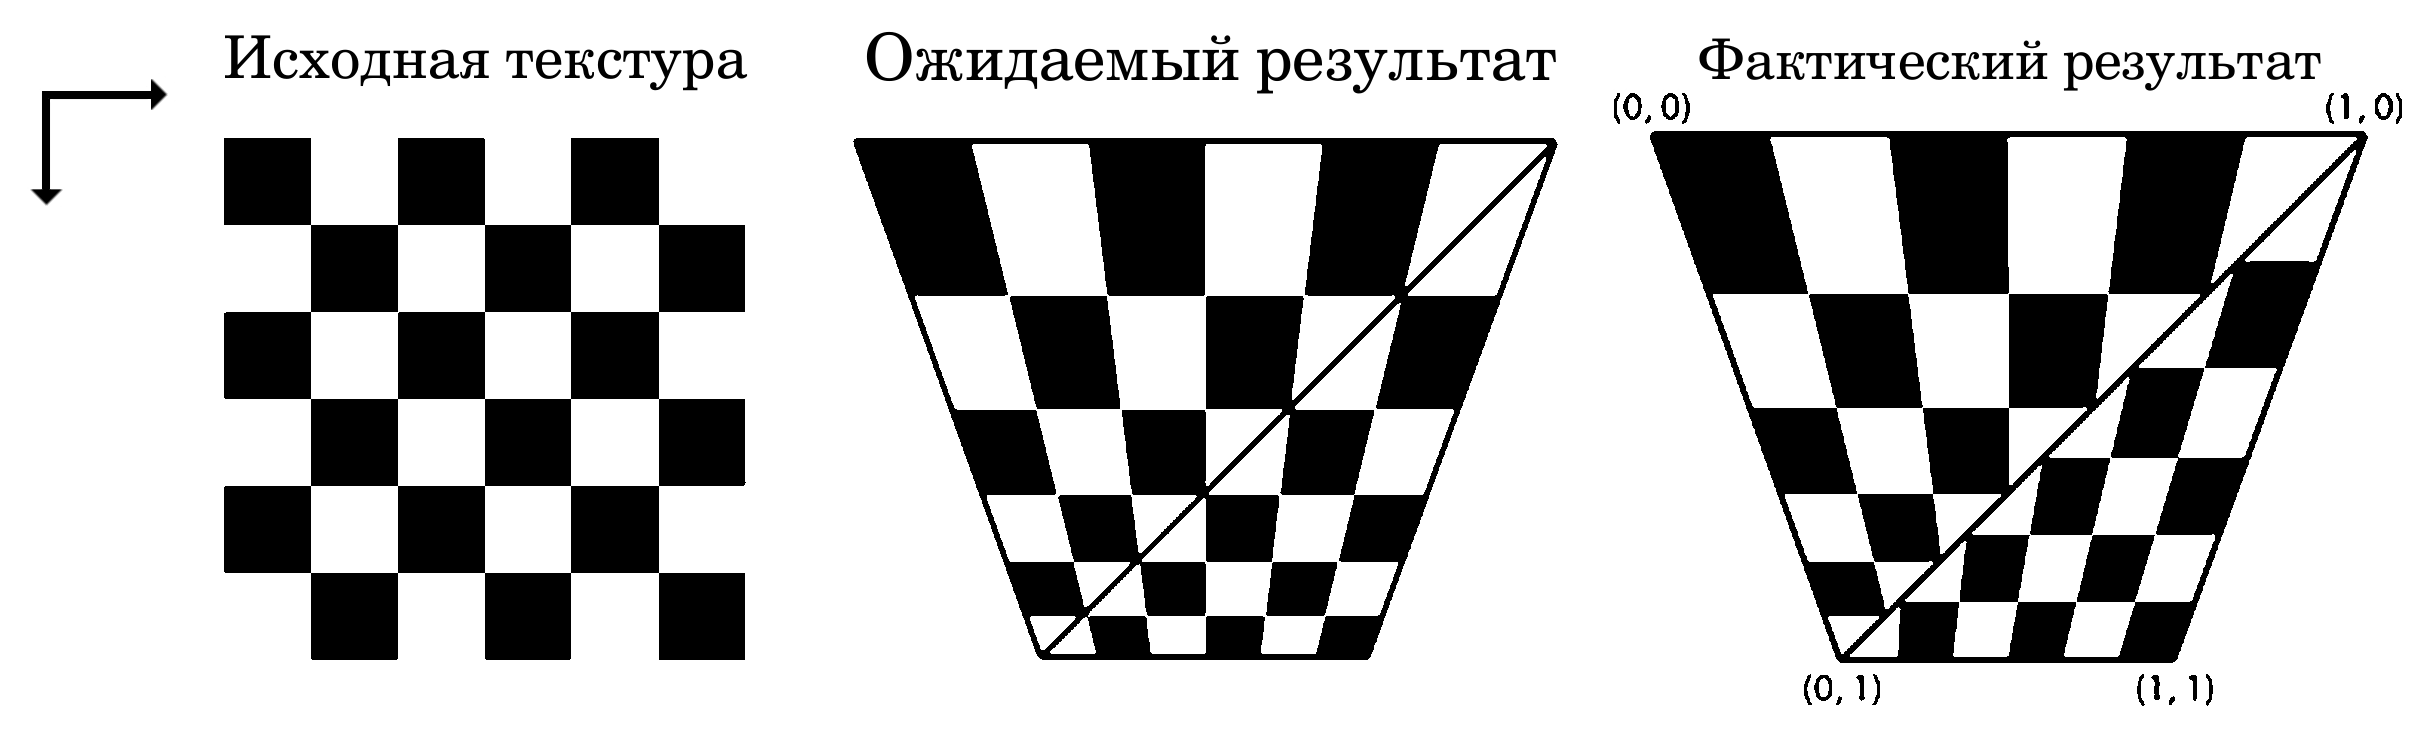
\includegraphics[width=\textwidth]{affine.png}
	\caption{Искажение изображения при кусочном афинном искривлении}
	\label{fig:affine}
\end{figure}

Для борьбы с этим эффектом используются различные техники, одна из них описывается в статье Schaefer, 2006 \cite{warping}, и именно этот подход используется в данной работе для искривления по ключевым точкам.

\subsection{Эксперименты с методами выравнивания}

В ходе реализации системы имитации возраста было решено сосредоточиться на проблеме выравнивания лица, т.е. приведения изображения лица к нейтральному виду. Дело в том, что от того, насколько точно решена эта задача, зависит то, насколько точно будут наложены текстурные изменения и изменения в оптическом потоке.

Поскольку авторы статьи Illumination-aware Age Progression прибегают к использованию собственного алгоритма Collection flow, решено было начать с него. По описанию из статьи была запрограммирована реализация на C++ с использованием библиотеки алгоритмов компьютерного зрения OpenCV. 
Алгоритм этот хоть и предназначен для вычисления оптического потока, вполне пригоден и для нейтрализации выражения лица, поскольку использует для этого промежуточное искривление исходного лица до его проекции.

Для экспериментов был взят тот же самый набор изображений лиц Adience \cite{adience}, содержащий 3210 лиц людей разного пола и возраста (на иллюстрациях <<all>>). Дополнительно были отобраны 309 фотографий одного и того же человека для проверки алгоритма в условиях, описанных в статье: когда задана большая выборка фотографий одного и того же человека (на иллюстрациях <<id>>).

Первоначально на вход алгоритму подавались фотографии, кадрированные до прямоугольника, содержащего лицо безо всякой другой предобработки. Первые результаты (см. рис. \ref{fig:exp_no}) показали, что предобработка, а именно какой-то дополнительный метод выравнивания лица, необходима: среднее изображение после работы collection flow оказалось неотличимо от среднего изображения до работы collection flow.

\begin{figure}[t]
\centering
	\begin{subfigure}[t]{0.3\textwidth}
		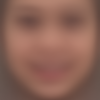
\includegraphics[width=\textwidth]{results/all_no_mean.png}
		\caption{all, 15.606}
	\end{subfigure}
	\begin{subfigure}[t]{0.3\textwidth}
		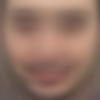
\includegraphics[width=\textwidth]{results/id2_no_mean.png}
		\caption{id, 21.1797}
	\end{subfigure}
	\caption{Collection flow: средние магнитуды для средних изображений по all и id}
	\label{fig:exp_no}
\end{figure}


Было решено добавить этап фронтализации перед вызовом collection flow. Основываясь на оригинальной Matlab-реализации, была создана собственная реализация данного подхода на С++ и OpenCV. В процессе разработки выяснилось, что алгоритм фронтализации был адаптирован для изображений в низком разрешении, в результате на изображениях большого разрешения оставались характерные артефакты в виде сетки (см. рис. \ref{fig:exp_err}). Решено было исправить эту проблему, во-первых, за счёт интерполяции точек в модели с разрешения $320 \times 320$ до $640 \times 640$, во-вторых, за счёт использования дилатации.

\begin{figure}[t]
\centering
	\begin{subfigure}[t]{0.3\textwidth}
		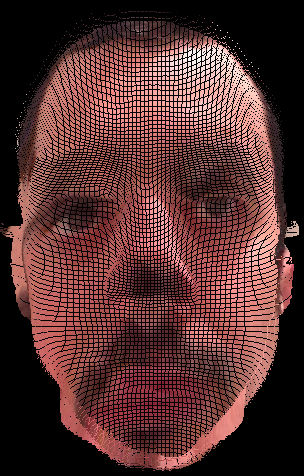
\includegraphics[width=\textwidth]{bad_model_reprojection.png}
		\caption{до дилатации}
	\end{subfigure}
	\begin{subfigure}[t]{0.3\textwidth}
		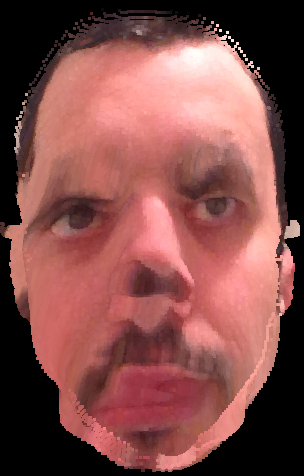
\includegraphics[width=\textwidth]{bad_model_dilatation.png}
		\caption{после дилатации}
	\end{subfigure}
	\begin{subfigure}[t]{0.3\textwidth}
		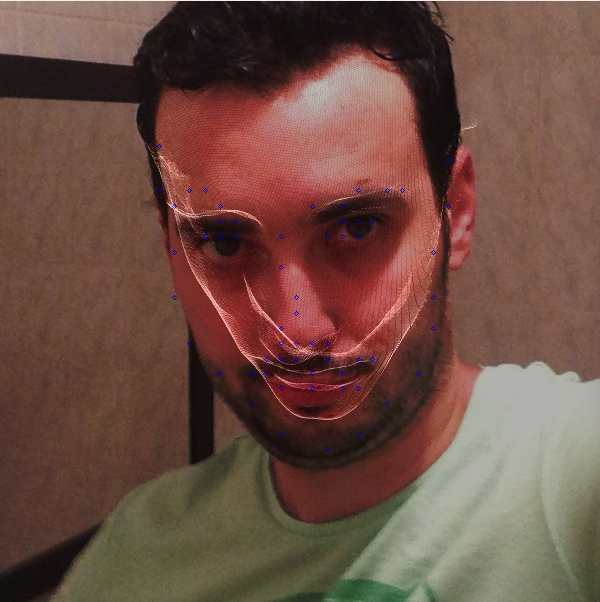
\includegraphics[width=\textwidth]{bad_model_fitting.png}
		\caption{неверная поза модели}
	\end{subfigure}
	\caption{Ошибки фронтализации}
	\label{fig:exp_err}
\end{figure}

В качестве детектора точек использовался детектор от Jason Saragin, реализованный в CSIRO Face Analysis SDK.

Также выяснилась ещё одна проблема: детектор ключевых точек от Jason Saragih плохо приспособлен к работе с неподвижными изображениями, основное его предназначение --- работа с живым видео, когда детектор улучшает свой результат от кадра к кадру. Из-за неточного соответствия ключевых точек особенностям лица поза для трёхмерной модели была найдена неправильно, в результате <<фронтализованное>> лицо теряло свои черты и искажалось (см. рис. \ref{fig:exp_err}), из-за чего точность выравнивания снижалась (см. рис. \ref{fig:exp_js}).

\begin{figure}[b]
\centering
	\begin{subfigure}[t]{0.3\textwidth}
		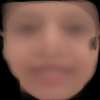
\includegraphics[width=\textwidth]{results/all_myfront_mean.png}
		\caption{all, 35.9171}
	\end{subfigure}
	\begin{subfigure}[t]{0.3\textwidth}
		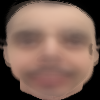
\includegraphics[width=\textwidth]{results/id2_myfront_mean.png}
		\caption{id, 50.6863}
	\end{subfigure}
	\caption{Фронтализация с детектором Jason Saragih: средние магнитуды для средних изображений по all и id}
	\label{fig:exp_js}
\end{figure}

\begin{figure}[h]
\centering
	\begin{subfigure}[t]{0.3\textwidth}
		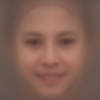
\includegraphics[width=\textwidth]{results/all_front_mean.png}
		\caption{all, 17.6375}
	\end{subfigure}
	\begin{subfigure}[t]{0.3\textwidth}
		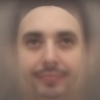
\includegraphics[width=\textwidth]{results/id2_front_mean.png}
		\caption{id, 30.9887}
	\end{subfigure}
	\caption{Фронтализация с детектором Zhu Ramanan: средние магнитуды для средних изображений по all и id}
	\label{fig:exp_zr}
\end{figure}

\begin{figure}[h]
\centering
	\begin{subfigure}[t]{0.3\textwidth}
		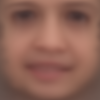
\includegraphics[width=\textwidth]{results/all_warped_mean.png}
		\caption{all, 20.8787}
	\end{subfigure}
	\begin{subfigure}[t]{0.3\textwidth}
		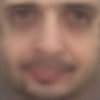
\includegraphics[width=\textwidth]{results/id2_warped_mean.png}
		\caption{id, 27.0529}
	\end{subfigure}
	\caption{Искривление по ключевым точкам: средние магнитуды для средних изображений по all и id}
	\label{fig:exp_warp}
\end{figure}

Следующей модификацией решено было, как и в оригинальной реализации, использовать из трёхмерной модели не только голову, но и фон, чтобы избавиться от дополнительных артефактов на границе лица. Кроме того, был использован детектор ключевых точек за авторством Zhu, Ramanan.

Средние изображения демонстрируют очень точное совпадение черт лица (см. рис. \ref{fig:exp_zr}), даже несмотря на то, что никакого специального выравнивания по чертам лица не проводилось. Более того, хотя детектор Zhu, Ramanan в силу особенностей HOG ограничен точностью в 8 пикселей, это не помешало ему справиться со своей задачей лучше, чем детектор от Jason Saragih, не имеющий такого ограничения в точности.

Следующий эксперимент состоял в использовании искривления по ключевым точкам для повышения точности. Для детектирования использовался детектор Zhu, Ramanan, показавший свою более высокую точность.

Данный метод не оправдал надежд, возложенных на него: пропорции лица существенным образом искажены (см. рис. \ref{fig:exp_warp}), что особенно заметно на среднем изображении для единственного человека.

Таким образом, из всех перечисленных методов выравнивания лица наибольшую эффективность показал метод фронтализации, выполненный по оригинальной схеме с детектором Zhu, Ramanan. Также оказалось, что метрика среднего градиента плохо описывает качество работы методов выравнивания: на изображениях с детектора Jason Saragin эта метрика из-за артефактов по краям была слишком большой; в то же время метрика не смогла показать, что искривление по ключевым точкам ухудшает результат, искажая пропорции лица.

Что до collection flow, то ни одна из описанных выше техник не позволила методу улучшить результат по сравнению со входными данными. В лучшем случае на выходе collection flow выдаёт неотличимое от входного среднее, в худшем --- портит результат, размывая изображения, что показывает низкую эффективность данного метода в решении задачи выравнивания лица.